\documentclass[12pt,twoside]{article}
\usepackage{indentfirst}
\usepackage[nottoc]{tocbibind}
\usepackage{fancyhdr,ragged2e}
\usepackage{todonotes}
\fancyhead{}
%%%%%%%%%%%%%%%%%%%%%%%%%%%%%%%%%%%%%%%%%%%%%%%%%%%%%%%%%%%%%%%%%%%%%%%%%%%%%

% Definitions for the title page
% Edit these to provide the correct information
% e.g. \newcommand{\reportauthor}{Timothy Kimber}

\newcommand{\reporttitle}{Evaluating the Use of Machine Learning for Doubly-Robust Estimation in Missing Data}
\newcommand{\reportauthor}{Juliette Maiko Limozin}
\newcommand{\supervisor}{Dr David Whitney}
\newcommand{\degreetype}{Mathematics}
\newcommand{\expit}{\text{expit}}
%%%%%%%%%%%%%%%%%%%%%%%%%%%%%%%%%%%%%%%%%%%%%%%%%%%%%%%%%%%%%%%%%%%%%%%%%%%%%

% load some definitions and default packages
%%%%%%%%%%%%%%%%%%%%%%%%%%%%%%%%%%%%%%%%%
% University Assignment Title Page 
% LaTeX Template
% Version 1.0 (27/12/12)
%
% This template has been downloaded from:
% http://www.LaTeXTemplates.com
%
% Original author:
% WikiBooks (http://en.wikibooks.org/wiki/LaTeX/Title_Creation)
%
% License:
% CC BY-NC-SA 3.0 (http://creativecommons.org/licenses/by-nc-sa/3.0/)
% 
%
%%%%%%%%%%%%%%%%%%%%%%%%%%%%%%%%%%%%%%%%%
%----------------------------------------------------------------------------------------
%	PACKAGES AND OTHER DOCUMENT CONFIGURATIONS
%----------------------------------------------------------------------------------------
\usepackage[a4paper,hmargin=2.5cm,vmargin=2.5cm,includeheadfoot]{geometry}
\usepackage{textpos}
\usepackage{natbib} % for bibliography
\usepackage{tabularx,longtable,multirow,subfigure,caption}%hangcaption
\usepackage{fncylab} %formatting of labels
\usepackage{fancyhdr} % page layout
\usepackage{url} % URLs
\usepackage[english]{babel}
\usepackage{amsmath}
\usepackage{graphicx}
\usepackage{dsfont}
\usepackage{epstopdf} % automatically replace .eps with .pdf in graphics
\usepackage{backref} % needed for citations
\usepackage{array}
\usepackage{latexsym}
\usepackage[pdftex,pagebackref,hypertexnames=false,colorlinks]{hyperref} % provide links in pdf

\hypersetup{pdftitle={},
  pdfsubject={}, 
  pdfauthor={},
  pdfkeywords={}, 
  pdfstartview=FitH,
  pdfpagemode={UseOutlines},% None, FullScreen, UseOutlines
  bookmarksnumbered=true, bookmarksopen=true, colorlinks,
    citecolor=black,%
    filecolor=black,%
    linkcolor=black,%
    urlcolor=black}

\usepackage[all]{hypcap}


%\usepackage{color}
%\usepackage[tight,ugly]{units}
%\usepackage{float}
%\usepackage{tcolorbox}
%\usepackage[colorinlistoftodos]{todonotes}
% \usepackage{ntheorem}
% \theoremstyle{break}
% \newtheorem{lemma}{Lemma}
% \newtheorem{theorem}{Theorem}
% \newtheorem{remark}{Remark}
% \newtheorem{definition}{Definition}
% \newtheorem{proof}{Proof}


%%% Default fonts
\renewcommand*{\rmdefault}{bch}
\renewcommand*{\ttdefault}{cmtt}



%%% Default settings (page layout)
\setlength{\parindent}{0em}  % indentation of paragraph

\setlength{\headheight}{14.5pt}

\fancyfoot[ER,OL]{\sffamily\textbf{\thepage}}%Page no. in the left on odd pages and on right on even pages
\fancyfoot[OC,EC]{\sffamily }
\renewcommand{\headrulewidth}{0.1pt}
\renewcommand{\footrulewidth}{0.1pt}
\captionsetup{margin=10pt,font=small,labelfont=bf}


%--- chapter heading

\def\@makechapterhead#1{%
  \vspace*{10\p@}%
  {\parindent \z@ \raggedright \sffamily
    \interlinepenalty\@M
    \Huge\bfseries \thechapter \space\space #1\par\nobreak
    \vskip 30\p@
  }}

%---chapter heading for \chapter*  
\def\@makeschapterhead#1{%
  \vspace*{10\p@}%
  {\parindent \z@ \raggedright
    \sffamily
    \interlinepenalty\@M
    \Huge \bfseries  #1\par\nobreak
    \vskip 30\p@
  }}

\allowdisplaybreaks

% load some macros
% Here, you can define your own macros. Some examples are given below.

\newcommand{\R}[0]{\mathds{R}} % real numbers
\newcommand{\Z}[0]{\mathds{Z}} % integers
\newcommand{\N}[0]{\mathds{N}} % natural numbers
\newcommand{\C}[0]{\mathds{C}} % complex numbers
\renewcommand{\vec}[1]{{\boldsymbol{{#1}}}} % vector
\newcommand{\mat}[1]{{\boldsymbol{{#1}}}} % matrix


\date{October 2020}

\begin{document}

% load title page
% Last modification: 2015-08-17 (Marc Deisenroth)
\begin{titlepage}

\newcommand{\HRule}{\rule{\linewidth}{0.5mm}} % Defines a new command for the horizontal lines, change thickness here


%----------------------------------------------------------------------------------------
%	LOGO SECTION
%----------------------------------------------------------------------------------------


\includegraphics[width = 4cm]{./figures/imperial}\\[0.5cm] 

\center % Center remainder of the page

%----------------------------------------------------------------------------------------
%	HEADING SECTIONS
%----------------------------------------------------------------------------------------

\textsc{\Large Imperial College London}\\[0.5cm] 
\textsc{\large Department of Mathematics}\\[0.5cm] 

%----------------------------------------------------------------------------------------
%	TITLE SECTION
%----------------------------------------------------------------------------------------

\HRule \\[0.4cm]
{ \huge \bfseries \reporttitle}\\ % Title of your document
\HRule \\[1.5cm]
 
%----------------------------------------------------------------------------------------
%	AUTHOR SECTION
%----------------------------------------------------------------------------------------

\begin{minipage}{0.4\textwidth}
\begin{flushleft} \large
\emph{Author:}\\
\reportauthor % Your name
\end{flushleft}
\end{minipage}
~
\begin{minipage}{0.4\textwidth}
\begin{flushright} \large
\emph{Supervisor:} \\
\supervisor % Supervisor's Name
\end{flushright}
\end{minipage}\\[4cm]


%----------------------------------------------------------------------------------------
%	FOOTER & DATE SECTION
%----------------------------------------------------------------------------------------
\vfill % Fill the rest of the page with whitespace
Submitted in partial fulfillment of the requirements for the MSci degree in
\degreetype~of Imperial College London\\[0.5cm]

\makeatletter
\@date 
\makeatother


\end{titlepage}



% page numbering etc.
\pagenumbering{roman}
\clearpage{\pagestyle{empty}\cleardoublepage}
\setcounter{page}{1}
\pagestyle{fancy}
\setlength{\parindent}{5ex}
%%%%%%%%%%%%%%%%%%%%%%%%%%%%%%%%%%%%
\begin{abstract}
\todo[inline]{to do once I have all results}


\end{abstract}

\clearpage
%%%%%%%%%%%%%%%%%%%%%%%%%%%%%%%%%%%%
\section*{Acknowledgments}
I would like to thank my project supervisor, Dr David Whitney, for his continued guidance and support throughout this project. Our weekly meetings have always been a pleasure, and his advice on postgraduate studies have also been of immense help. 

I would also like to thank my family, who even though might not understand Statistics at a Master's level, have always enabled me to achieve my best.

Last but not least, I would like to thank my various statistics lecturers who, in my 4 years at Imperial, have enamoured me with their passion for Statistics.

\clearpage{\pagestyle{empty}\cleardoublepage}

%%%%%%%%%%%%%%%%%%%%%%%%%%%%%%%%%%%%
%--- table of contents
\tableofcontents 


\clearpage
\pagenumbering{arabic}
\setcounter{page}{1}
\fancyhead[L]{\textsl{\leftmark}}

\setcitestyle{authoryear,open={(},close={)}}
%%%%%%%%%%%%%%%%%%%%%%%%%%%%%%%%%%%%
\section{Introduction} 

Missing data is a common issue encountered in Statistics, and can have a significant effect on statistical inferences one may draw from the data. Suppose one wishes to estimate the mean outcome value of a data set that has some missing outcome values. One way to approach this issue is to simply discard the data points that do not have an outcome value accounted for, but that would be a loss of valuable feature information we still have of these data points, and this estimation would likely be biased.

Many bias-minimising strategies exist for estimating the mean outcome value. The most efficient method consists of fitting predictive models of the outcome and 'missingness' pattern, and use the fitted values as part of the outcome mean calculation. Such a way of estimating the outcome mean is called the augmented inverse probability weighting (AIPW) approach, often referred to as doubly-robust (DR) estimation. This approach has been popularised in many fields, as it provides the user two chances of maintaining consistency, as only one of the two predictive models needs to be correctly specified. The art of specifying these models, however, is the biggest challenge one has to face when using DR estimation. We wish to consider models that are not only accurate but also provide a DR estimate whose bias converges to 0 at a rate faster than that of $N^{-1/2}$, which is generally the rate of convergence to the true value that we aim for in statistical literature.

Traditionally, parametric models are used to predict the outcome and the probability of observing the outcome given the feature data (referred to as propensity score). As parametric models form a family of probability distributions, their parameter range is finite and they provide useful theoretical backings such as the ability to infer on asymptotic distributions and confidence intervals (CIs). However a slight misspecification can lead to biased estimates. In recent years, developments in data-adaptive non-parametric tools make one consider these Machine Learning (ML) approaches, and whether or not they are more efficient at fitting the predictive models correctly even with a slight misspecification, which would benefit DR estimation.
 
In this report we will illustrate the use of DR estimation, starting with a parametric setting that includes DR estimates with one or more misspecified models. We will then move towards flexible nonparametric methods, notably Random Forests (RFs) and Multilayer Perceptrons (MLPs), to see if they provide improved inference while still maintaining consistent estimation. As we shall demonstrate in section 3, parametric models are likely to be misspecified in practice and the misspecification leads to highly biased estimators with CIs eventually not containing the true value. In section 4, we suggest that flexible nonparametric methods such as RFs and MLPs provide more degrees of freedom to get a correct specification of the nuisance parameter models, but have difficulty reaching a high convergence rate of the bias, and CI constructed using nuisance parameter models-based SE estimation as suggested by \cite{davidian} also lead non-optimal rate of convergence to high coverage. \cite{benkeser2017} have proposed alternative correction procedures to provide DR estimators with almost-nominal CI coverage; however, the results presented in this report suggest that more research must be conducted on how to optimise hyperparameter tuning of such nonparametric methods in order reduce DR estimation bias.

\clearpage 
\section{Setting} 

Suppose we have a data set of size $n$, and realisations of random vector $(\mathbf{Y}, \mathbf{W}, \mathbf{R})$ where $\mathbf{Y}$ denotes a partially denoted outcome, i.e. $Y_i$ is missing for individual $i$'s unobserved outcome. $\mathbf{W}$ denotes the auxiliary variables, and $\mathbf{R}$ is an indicator on whether the $i$th individual's outcome is missing or not; that is, if $R_i = 1$, the outcome is observed, whereas $R_i = 0$ would indicate that the outcome is missing.
To summarise:
\begin{itemize}
    \item $\mathbf{Y}$: partially observed outcome 
    \item $\mathbf{W}$: auxiliary variables/covariates 
    \item $\mathbf{R}$: indicator on whether $Y$ is observed or not ($R = 1$: observed, $R = 0$: missing) 
\end{itemize}

The outcome is said to be \textbf{missing at random (MAR)} if the conditional probability that a particular missingness pattern occurs given the data is independent of the missing values in that pattern \citep{vansteelandt}, i.e $P(R=r|\mathbf{W}, Y) = P(R= r|\mathbf{W})$ and  $P(Y=y|\mathbf{W}, R) = P(Y=y|\mathbf{W})$. So in the example of a clinical trial, we would consider the data set obtained from the study to be MAR if given the measurements taken from the patients, the reasons why some patients dropped out were unrelated to the outcome of the trial. The MAR setting will therefore have effects on any statistical inference we may perform on this data set.

When the missingness pattern is independent of both the auxiliary variables and the outcome data, the data set is said to be \textbf{missing completely at random (MCAR)}.\\

We make the assumption that $(\mathbf{W}_1, Y_1, R_1),...,(\mathbf{W}_n, Y_n, R_n)$ are independent and identically distributed for the rest of the report. We also assume that $R$ is independent of $Y$ given $\mathbf{W}$ so $(\mathbf{W}_1, Y_1, R_1), ... ,(\mathbf{W}_n, Y_n, R_n)$ are MAR \citep{vansteelandt}, where the index $i = 1,...,n$ denotes the $i$th individual of the data.\\

\clearpage
\section{Non-robust and DR estimators}

\subsection{Inverse Probability Weighting approach}

Suppose we wish to calculate or estimate the outcome mean $\beta = E(\mathbf{Y})$. A problem occurs when trying to compute it as $\mathbf{Y}$ is only partially observed, so calculating a mean with only the observed outcomes would not be a good representation of the data outcome as a whole.

One solution to this problem is the inverse probability weighting (IPW) approach. Its name comes from the fact that each observed outcome $Y_i$ (called \textit{complete} case) is weighted by the propensity score, denoted by
\begin{align*}
    \pi(\mathbf{W})= E(R|\mathbf{W}) = P(R = 1|\mathbf{W}).
\end{align*}

We assume that the weighting is bounded away from 0 almost for any $\mathbf{W}_i$.

The IPW estimator of the mean $\beta$ is then simply 
\begin{equation} \label{IPW_est}
    \hat{\beta}_{IPW} = \frac{1}{n} \sum_{i=1}^{n} \frac{R_iY_i}{\pi(\mathbf{W}_i)}.
\end{equation}

In practice, the propensity score $\pi(\mathbf{W})$ is unknown, so we predict the probabilities using, most commonly, a parametric model $\hat\pi(\mathbf{W}; \boldsymbol\alpha)$ for the missingness pattern and we build an estimator $\hat{\boldsymbol\alpha}$ of $\boldsymbol\alpha$ from the data \citep{vansteelandt}.

If the propensity score model $\hat\pi(\mathbf{W}; \boldsymbol\alpha)$ is correctly specified, by the weak law of large numbers (WLLN), $\hat{\beta}_{IPW}$ will converge in probability to the true mean $\beta$, so this makes the IPW estimate consistent for $\beta$ \citep{davidian}. Using the Central Limit Theorem (CLT), we have $\sqrt{n}(\hat{\beta}_{IPW}-\beta) \xrightarrow{d} N(0,\sigma^2)$ where $\sigma$ is the estimated outcome variance (often a sample-based estimator in practice), so we can use this result to perform inference tests and CIs for the true mean.

A drawback from the IPW estimator in equation \ref{IPW_est} is that it is usually difficult to construct a propensity score model unless the auxiliary variables $\mathbf{W}$ are categorical or the sample size $n$ is large enough, so a removal of bias is not guaranteed by the IPW estimator when the model is misspecified. Another problem that arises is unstable weights: if the model is misspecified, the fitted probability of observing an outcome given the auxiliary variables may be very small for the majority of individuals, and very large for a select few, so the IPW estimator is mainly dominated by these large weights \citep{seaman}.

\citet{kang} suggest that the model being misspecified is more likely the cause of large weights, rather than if the auxiliary variables are truly predictive of whether the outcome may be missing or not. There exist a few tests, including the \citet{hosmer} test, to detect poor fit of the propensity score model.\\

\subsection{Regression imputation approach} 

Alternatively, one could make use of the conditional expectation of the outcome 
\begin{align*}
    m(\mathbf{W}) = E(Y|R= 1,\mathbf{W})
\end{align*}
to have a different estimator of the mean \citep{davidian,vansteelandt}, sometimes called the regression imputation estimator: 

\begin{equation}
    \hat{\beta}_ {RI} = \frac{1}{n}\sum_{i = 1}^n m(\mathbf{W}_i)
\end{equation}

In practice the true value of $m(\mathbf{W})$ is unknown, we propose an outcome model, most commonly a parametric model $\hat m(\mathbf{W}, \gamma)$ with some parameter $\gamma$, and again we build an estimator $\hat{\gamma}$ for $\gamma$ from the sample data. Like in IPW, the efficiency of the RI estimator in terms of consistency relies on the correct specification of the outcome model, as then the WLLN would apply and so the RI estimator would be consistent for $\beta$. \\

\subsection{Augmented IPW approach} 

The estimation strategies from the previous sections motivate the idea behind the AIPW estimator. One could think of combining the ideas from the IPW and RI estimators. From \citet{davidian}, IPW estimators of $\beta$, when the propensity score model is correctly specified and the estimators are consistent and are asymptotically normal (i.e. CLT holds), are equivalent to 

\begin{equation}
    \frac{1}{n}\sum_{i=1}^{n}\frac{R_iY_i}{\hat\pi(\mathbf{W}_i, \hat{\alpha})} - \frac{1}{n}\sum_{i=1}^{n} \left(1 - \frac{R_i}{\hat\pi(\mathbf{W_i},\hat{\alpha})} \right) h(\mathbf{W}_i)
\end{equation}

This is called an AIPW as it is the sum of the IPW estimator and an augmentation term depending on $h(\mathbf{W})$ \citep{davidian}. By taking $-h(\mathbf{W}) = \hat m(\mathbf{W}, \hat{\gamma})$ like in the RI approach, we have a new estimator
\begin{equation}
    \hat\beta_{DR} = \frac{1}{n}\sum_{i=1}^{n}\frac{R_iY_i}{\hat \pi(\mathbf{W}_i, \hat{\alpha})} + \frac{1}{n}\sum_{i=1}^{n} \left(1 - \frac{R_i}{\hat\pi(\mathbf{W_i},\hat{\alpha})} \right) \hat m(\mathbf{W}_i, \hat\gamma)
\end{equation}

The estimator $\hat\beta_{DR}$ is consistent (i.e $\hat\beta_{DR}$ converges in probability to the true mean $\beta$) and asymptotically normal when either the propensity score or outcome model are correctly specified, as the correct specification of one suffices for consistency, and therefore the CLT to hold for $\hat\beta_{DR}$, which is why we call this a \textbf{DR estimator} for $\beta$. This allows us to not require a correct specification for the entire outcome ans missingness distributions whilst maintaining a better efficiency than IPW estimators \citep{bangrobins,vansteelandt}.

For example, DR estimators are used to estimate the mean of clinical trial outcome when there have been dropouts mid-trial; we use acquired variables/observations on patients to compute a DR estimation of the mean. \\

The proof of the double-robustness of this mean estimator is as follows, mainly taken from \citet{vansteelandt}.

Rewriting $\hat{\beta}_{DR}$, we have
\begin{align*}
    \hat{\beta}_{DR} & = \frac{1}{n}\sum_{i=1}^{n}\frac{R_iY_i}{\hat\pi(\mathbf{W}_i, \hat{\alpha})} + \frac{1}{n}\sum_{i=1}^{n} \left(1 - \frac{R_i}{\hat\pi(\mathbf{W_i},\hat{\alpha})} \right) \hat m(\mathbf{W}_i, \hat\gamma) \\
    & = \frac{1}{n}\sum_{i=1}^{n} Y_i + \frac{1}{n}\sum_{i=1}^{n}\left(1 - \frac{R_i}{\hat\pi(\mathbf{W_i},\hat{\alpha})} \right) (\hat m(\mathbf{W}_i, \hat\gamma)-Y_i)
\end{align*}

Using the WLLN, we have $\frac{1}{n}\sum_{i=1}^{n} Y_i\xrightarrow{p} E(Y_1) = \beta$. Hence the DR estimator is consistent for the true mean $\beta$ if the sum added to $\frac{1}{n}\sum_{i=1}^{n} Y_i$ converges in probability to 0. \\

\textbf{Case 1:} Suppose the propensity score $\hat\pi(\mathbf{W},\hat{\alpha})$ is correctly specified and $\hat{\alpha} \xrightarrow{p} \alpha$, therefore  $\hat\pi(\mathbf{W},\hat{\alpha}) \xrightarrow{p} \pi(\mathbf{W}) = E(R|\mathbf{W}) = E(R|\mathbf{W}, Y)$ under MAR assumption. Then using the tower rule on expectations, we have
\begin{align*}
& \frac{1}{n}\sum_{i=1}^{n}\left(1 - \frac{R_i}{\hat\pi(\mathbf{W_i},\hat{\alpha})} \right) (\hat m(\mathbf{W}_i, \hat\gamma)-Y_i) \\
     & \phantom{E [(1 - \frac{R_1}{\pi(\mathbf{W_1})})} \xrightarrow{p} E \left[\left(1 - \frac{R_1}{\pi(\mathbf{W_1})} \right) (\hat m(\mathbf{W}_1, \hat\gamma)-Y_1)\right]  \\
     & \phantom{E [(1 - \frac{R_1}{\pi(\mathbf{W_1})})} = E\left[E\left[\left(1 - \frac{R_1}{\pi(\mathbf{W_1})} \right) (\hat m(\mathbf{W}_1, \hat\gamma)-Y_1)|Y_1, \mathbf{W}_1\right]\right] \\
     & \phantom{E [(1 - \frac{R_1}{\pi(\mathbf{W_1})})} = E\left[ (\hat m(\mathbf{W}_1, \hat\gamma)-Y_1)E\left[\left(1 - \frac{R_1}{\pi(\mathbf{W_1})} \right)|Y_1, \mathbf{W}_1\right]\right] \\
     & \phantom{E [(1 - \frac{R_1}{\pi(\mathbf{W_1})})} = E\left[ (\hat m(\mathbf{W}_1, \hat\gamma)-Y_1)\left(1 - \frac{E(R_1|Y_1, \mathbf{W}_1)}{\pi(\mathbf{W_1})} \right)\right] \\
     & \phantom{E [(1 - \frac{R_1}{\pi(\mathbf{W_1})})} = E\left[ (\hat m(\mathbf{W}_1, \hat\gamma)-Y_1)\left(1 - \frac{E(R_1|Y_1, \mathbf{W}_1)}{E(R_1|Y_1, \mathbf{W}_1)} \right)\right] \\
     &  \phantom{E [(1 - \frac{R_1}{\pi(\mathbf{W_1})})} = 0
\end{align*}
Hence $\hat{\beta}_{DR} \xrightarrow{p} \beta$. \\

\textbf{Case 2:} Suppose the outcome model $\hat m(\mathbf{W}, \hat\gamma)$ is correctly specified and $\hat{\gamma} \xrightarrow{p} \gamma$, therefore  $\hat m(\mathbf{W}, \hat\gamma) \xrightarrow{p} m(\mathbf{W}) = E(Y|R = 1,\mathbf{W})$ under MAR assumption. Then in a similar manner to case 1, we have
\begin{align*}
& \frac{1}{n}\sum_{i=1}^{n}\left(1 - \frac{R_i}{\hat\pi(\mathbf{W_i},\hat{\alpha})} \right) (\hat m(\mathbf{W}_i, \hat\gamma)-Y_i) \\
     & \phantom{E [(1 - \frac{R_1}{\pi(\mathbf{W_1})})} \xrightarrow{p} E\left[\left(1 - \frac{R_1}{\hat\pi(\mathbf{W_1},\hat{\alpha})} \right) (m(\mathbf{W}_1)-Y_1)\right]  \\
     & \phantom{E [(1 - \frac{R_1}{\pi(\mathbf{W_1})})} = E\left[ E\left[\left(1 - \frac{R_1}{\hat\pi(\mathbf{W_1},\hat{\alpha})} \right)(m(\mathbf{W}_1)-Y_1)|R_1 = 1, \mathbf{W}_1\right]\right] \\
     & \phantom{E [(1 - \frac{R_1}{\pi(\mathbf{W_1})})} = E\left[\left(1 - \frac{R_1}{\hat\pi(\mathbf{W_1},\hat{\alpha})} \right) E\left[(m(\mathbf{W}_1)-Y_1)|R_1 = 1, \mathbf{W}_1\right]\right] \\
     & \phantom{E [(1 - \frac{R_1}{\pi(\mathbf{W_1})})} = E\left[\left(1 - \frac{R_1}{\hat\pi(\mathbf{W_1},\hat{\alpha})} \right) (m(\mathbf{W}_1)-E\left[Y_1|R_1 = 1, \mathbf{W}_1\right])\right] \\
     & \phantom{E [(1 - \frac{R_1}{\pi(\mathbf{W_1})})} = E\left[\left(1 - \frac{R_1}{\hat\pi(\mathbf{W_1},\hat{\alpha})} \right) (E\left[Y_1|R_1=1, \mathbf{W}_1\right]-E\left[Y_1|R_1=1, \mathbf{W}_1\right])\right] \\
     & \phantom{E [(1 - \frac{R_1}{\pi(\mathbf{W_1})})} = 0
\end{align*}
Hence $\hat{\beta}_{DR} \xrightarrow{p} \beta$.\\

Thus we have shown that when at least one of the two models is correctly specified, the DR estimator is consistent for the true mean. It follows naturally that if both models are correctly specified, this result still holds.

\subsection{Parametric DR estimation}

In standard parametric DR estimation, it is fairly common to define the propensity and outcome models as logistic or linear regression models. These methods are user-friendly and fairly easy to understand and compute, as many pre-made functions are available in coding languages. They also offer theoretical backing that would allow us to make statistical inference.\\

Although this version of the DR estimator that these models lead to has been established as the usual estimator, \cite{kang} have shown it performs poorly when either the propensity or both models are misspecified, i.e when logistic and linear regressions aren't the judicious choice of models for the data. This gives no guarantee that $\hat\beta_{DR}$ is at least as efficient as the IPW estimator, which we were seeking to improve on.

Another issue with parametric DR estimators is that $\hat\beta_{DR}$ may be outside the range of the observed $\mathbf{Y}$ values; it could lie below or above the minimum or maximum value of $Y$, which would not be useful. This is especially true when we may have binary outcome \citep{vansteelandt}.

\subsection{Simulation study of parametric DR}
\label{para_model}

Let us look at an example to illustrate the use of parametric DR estimators. We take the model specification from \citet{benkeser2017}: our co-variate vector is $\mathbf{W} = (W_1, W_2)$, where $W_1$ is uniformly distributed over $[-2,2]$ and $W_2$ has a Bernoulli distribution of success probability $1/2$. $W_1$ and $W_2$ are independent. The missingness indicator $R$ is a Bernoulli random variable of success probability $\expit(-w_1 + 2w_1w_2)$. The true propensity score is therefore
\begin{align*}
    \pi(\mathbf{W}) = P(R = 1 |\mathbf{W} = (w_1,w_2)) = \expit(-w_1 + 2w_1w_2)
\end{align*}

The partially observed outcome has a conditional probability of occurrence 
\begin{align*}
    P(Y = 1|R = r,\mathbf{W} = (w_1, w_2)) = \expit(0.2r - w_1 + 2w_1w_2)
\end{align*}

The true outcome model is then 
\begin{align*}
    m(\mathbf{W}) = E(Y|\mathbf{W}, R=1) &= P(Y = 1|\mathbf{W}, R= 1) \\
    & = \expit(0.2 - w_1 + 2w_1w_2)
\end{align*}

From there we calculated four parametric DR estimates: 
\begin{itemize}
    \item \texttt{DR logistic models}, where the propensity score and outcome models are correctly specified by logistic regression fits that account for the interaction term between $W_1, W_2$;
    \item \texttt{DR exact specification}, where both models are correctly specified using the exact formulas above;
    \item \texttt{DR mis. outcome model}, where the outcome model is incorrectly specified by not accounting for the interaction term between $W_1, W_2$ in the logistic regression fit;
    \item \texttt{DR mis. propensity score}, where the propensity score model is incorrectly specified by not accounting for the interaction term between $W_1, W_2$ in the logistic regression fit.
    \item \texttt{DR misspecified}, where both the propensity score model and  is incorrectly specified by not accounting for the interaction term between $W_1, W_2$ in the logistic regression fit.
\end{itemize}

For each estimate we considered sample sizes $N = 200, 400, 600, ..., 2000$ and for each N we calculated the empirical bias of the estimators over 2500 generated data sets, as well as the empirical coverage of the 95\% CIs and accuracy of the standard error (SE) estimation from \citet{lunceford_davidian}.

By using properties of iterated expetations, we have

\begin{align*}
    E(Y|R = 1) &= P(Y = 1|R = 1)\\
    &= \int_{-2}^{2} \sum_{w_2 = 0}^{1} P(Y = 1, W_1 = w_1, W_2 = w_2|R = 1) dw_1 \\
    & = \int_{-2}^{2} \sum_{w_2 = 0}^{1} P(Y = 1|W_1 = w_1, W_2 = w_2, R = 1) \\
    & \phantom{ = \int_{-2}^{2} \sum_{w_2 = 0}^{1}} \cdot P(R = 1, W_1 = w_1, W_2 = w_2)dw_1 \\
    & = \int_{-2}^{2} \sum_{w_2 = 0}^{1} \expit(0.2 - w_1 + 2w_1w_2)P(R = 1|W_1 = w_1, W_2 = w_2) \\
    &\phantom{ = \int_{-2}^{2} \sum_{w_2 = 0}^{1}} \cdot P(W_1 = w_1)P(W_2 = w_2)dw_1 \\
    & = \int_{-2}^{2} \sum_{w_2 = 0}^{1} \expit(0.2 - w_1 + 2w_1w_2)\expit(-w_1+2w_1w_2) \cdot \frac{1}{4}\cdot \frac{1}{2}dw_1 \\
    & = \int_{-2}^{2} \frac{1}{8}[\expit(0.2 - w_1)\expit(-w_1) \\
    &\phantom{ = \int_{-2}^{2} \sum_{w_2 = 0}^{1}} +\expit(0.2 - w_1 + 2w_1)\expit(-w_1+2w_1)]dw_1 \\
    & = \int_{-2}^{2} \frac{1}{8}[\expit(0.2 - w_1)\expit(-w_1) +\expit(0.2 + w_1)\expit(w_1)]dw_1 \\
\end{align*}

By calculating the above integral numerically, we get that the true mean, had all outcome variables $Y_i$ been accounted for, is about 0.53.

For calculating the CIs, we set the model-based sample error estimates to be 
\begin{align*}
    \hat{SE} = n^{-1} \sqrt{\sum_{i=1}^n \left(\frac{R_i(Y_i - \hat m(\mathbf{W}_i), \hat \gamma)}{\hat\pi(\mathbf{W}_i,\hat\alpha)} + \hat m(\mathbf{W}_i) - \hat{\beta}_{DR}\right)^2}
\end{align*}
from \citet{lunceford_davidian}. \\

\subsubsection*{Results}

\begin{figure}[h!]
    \centering
    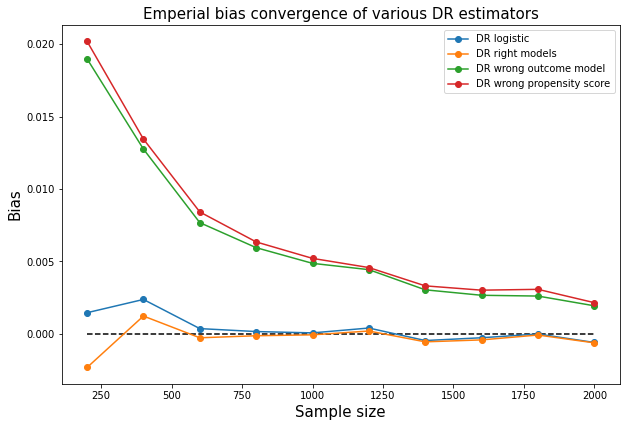
\includegraphics[width = 0.9\columnwidth]{figures/biaspara.png}
    \caption{Simulation results of bias for the various parametric DR estimator specifications}
    \label{figbiaspara}
\end{figure}

\begin{figure}[h!]
    \centering
    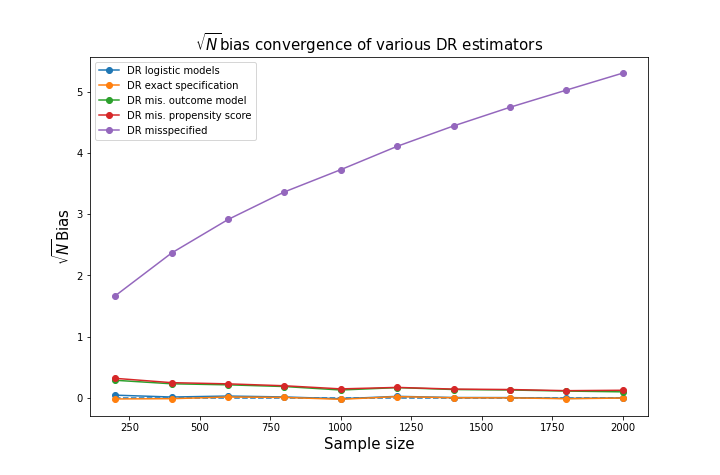
\includegraphics[width = 0.9\columnwidth]{figures/sqrtnpara.png}
    \caption{Simulation results of $\sqrt{N}$bias for the various parametric DR estimator specifications}
    \label{figsqrtnpara}
\end{figure}

Figure \ref{figbiaspara} suggests that the DR estimators with at least one correct specification of the nuisance parameter estimates are indeed consistent as the biases converge to 0 as the sample sizes $N$ get larger -- this is further illustrated in figure \ref{figsqrtnpara}, as we notice that the rates of convergence of the biases are faster than that of $N^{-1/2}$. We also notice that the DR estimation with wrong propensity score has the poorest convergence out of the 4 estimations, which is in line with the inefficiency that was suggested for such specifications by \citet{kang}. As expected, we also observe poor bias from the DR estimator with both nuisance parameter estimates misspecified, with a diverging $\sqrt{N}$bias curve, confirming that the misspecification of both parameters leads to inconsistent DR estimator.

\begin{figure}[h!]
    \centering
    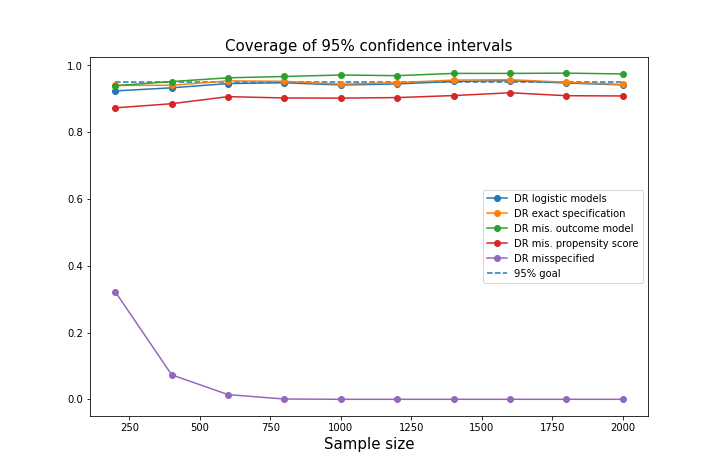
\includegraphics[width = 0.9\columnwidth]{figures/CIpara.png}
    \caption{Simulation results of 95\% CIs coverage for the various parametric DR estimator specifications}
    \label{figCIpara}
\end{figure}

\begin{figure}[h!]
    \centering
    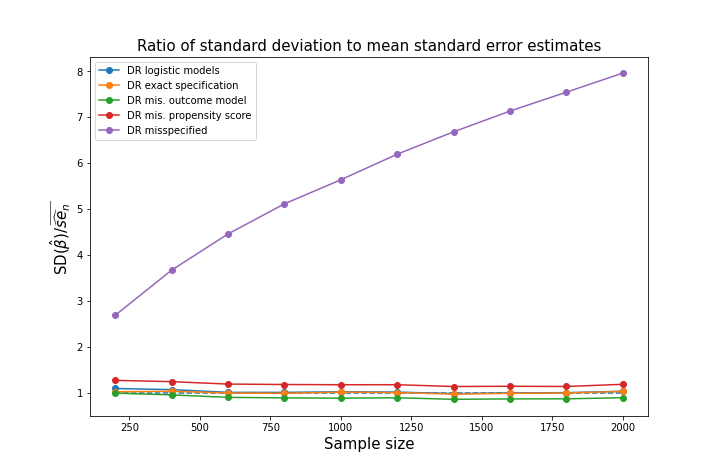
\includegraphics[width = 0.9\columnwidth]{figures/SEpara.png}
    \caption{Accuracy of \citet{lunceford_davidian} SE estimation for the various parametric DR estimator specifications}
    \label{figSEpara}
\end{figure}

Figure \ref{figCIpara} shows the empirical coverage of the 95\% CIs of each estimations, which indeed converge to 95\% for the correctly specified DR estimations. Because the estimation of the SE was specifically for correctly specified model, the coverage for the DR estimations with one wrong nuisance parameter are either too high or too low. To get a better estimation of the SE, one could try other non-model based methods such as bootstrapping, which calculates an estimate of the sample variance based on random samples of the DR estimates. On the flip-side, we notice that for the misspecified DR estimator, as expected the coverage of its CIs converge rapidly to 0, i.e. the CIs based on this misspecified estimator eventually don't contain the true value $\beta$.

Figure \ref{figSEpara} confirms the results we saw above, as we see the ratio of the standard deviation of the DR estimates to the average SE estimator is close to 1 for correctly specified models, hence suggesting a correct calculation of the CI bounds. As for the DR estimations with one wrong model, this ratio is above or below 1 for \texttt{DR mis. propensity score} and \texttt{DR mis. outcome model} respectively. This indicates that the SE estimation we used is positively or negatively biased, hence giving a CI coverage that is too low for the DR estimator with misspecified outcome model, or too high for the DR estimator with misspecified propensity score model. As for the standard deviation to mean SE estimate ratio for the misspecified DR estimator, since the SE estimation is based on correctly specified nuisance parameter estimates, it is to no surprise that it is inconsistent in this case, so the ratio diverges.

\begin{figure}[h!]
    \centering
    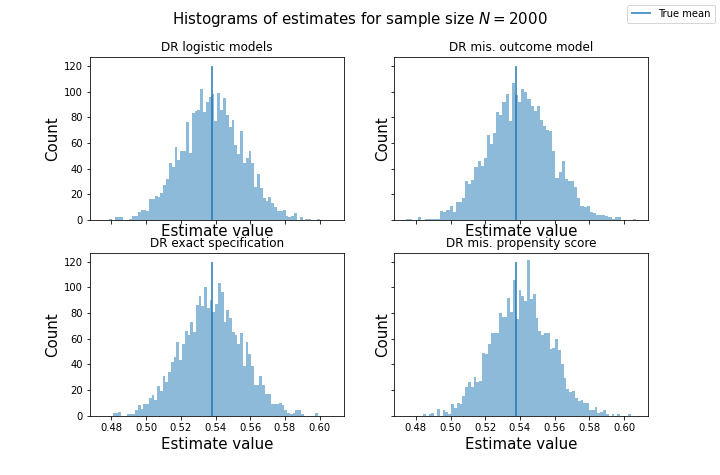
\includegraphics[width = 0.9\columnwidth]{figures/histpara.png}
    \caption{Histograms of parametric DR estimators from simulation results for sample size $N = 2000$}
    \label{fighistpara}
\end{figure}

Figure \ref{fighistpara} suggests that we indeed see asymptotic normality of the distribution, centered at the true mean, of the DR estimators that have at least one correctly specified nuisance parameter.\\

These results suggest that the parametric approach for setting the nuisance parameters is a good way of specifying these models, as shown by the consistency of the estimates. An important advantage of parametric DR estimation is the user-friendly aspect, as we have mentioned previously that logistic or linear regressions models are easy fitting methods to start with, and their theoretical results have been proven in the literature. However we were only able to set the models correctly because we knew the distribution of the data-generative method, and therefore the fact that there was an interactive term between $W_1,W_2$ in the logistic regression model. Had we been given this data set without any information on how it was generated, it would have been time-consuming to find the correct specification of at least one nuisance parameter. In practice we would be likely to see results as seen from the DR estimator with both models misspecified, which has no advantage as we saw the CIs eventually didn't contain the true mean. This is where the practicality of ensemble learners from ML tools seem to be a more efficient way of setting these models, which we will cover in the next section.

\clearpage
\section{ML approaches to optimise the DR estimator}

Parametric models for the propensity score and outcome regression are backed by many theoretical results in the literature, and are relatively simple models to train thanks to their finite parameter space. However we have seen in the simulation study above that even a slight misspecification can lead to biased estimations that have CIs almost surely not containing the true mean. Hence the convenience of parametric models is over-weighed by defectiveness under model misspecification \citep{diaz}.

Alternatively, one can use ML models to try to alleviate this bias and CI coverage, as they are often data-adaptive and therefore provide a certain degree of freedom to get a correctly specified model. In fact, \citet{ps_SL} have shown that when the propensity score is incorrectly specified, the use of ML tools for specifying the outcome regression can still give an unbiased DR estimator, which is an advantage over the parametric scenario, as we had seen that an incorrect propensity score with correct outcome regression was still giving the worse DR estimator in terms of bias in section \ref{para_model}.

Some data adaptive methods include: RFs, Support Vector Machines, kernel regression, outcome weighed learning, Q-learning, neural networks, ensembles of these methods, etc. These methods have been observed to have good empirical performance, but limited theoretical results exist for them. In the following sections we will take a closer look at the use of RFs and MLPs with various data settings, and see if these data-adaptive methods give better estimates compared to the results from parametric models, even accounting for higher model complexity by adding more covariates to the data.

\subsection{Using RFs}

RFs are a beginner friendly ML tool that create a classification or regression model based on multiple randomly generated decision trees that are combined together to make a better prediction than that of a single decision tree. It is easy to use and fit thanks to pre-existing packages in Python and R, and they are also capable of being trained on a dataset containing a mix of continuous and categorical features. However it is not the most time efficient tool, as the training of the models requires a non-negligible amount of computational power. In this section we will explore the use of RFs for fitting the nuisance parameters in DR estimation.

\begin{figure}
    \centering
    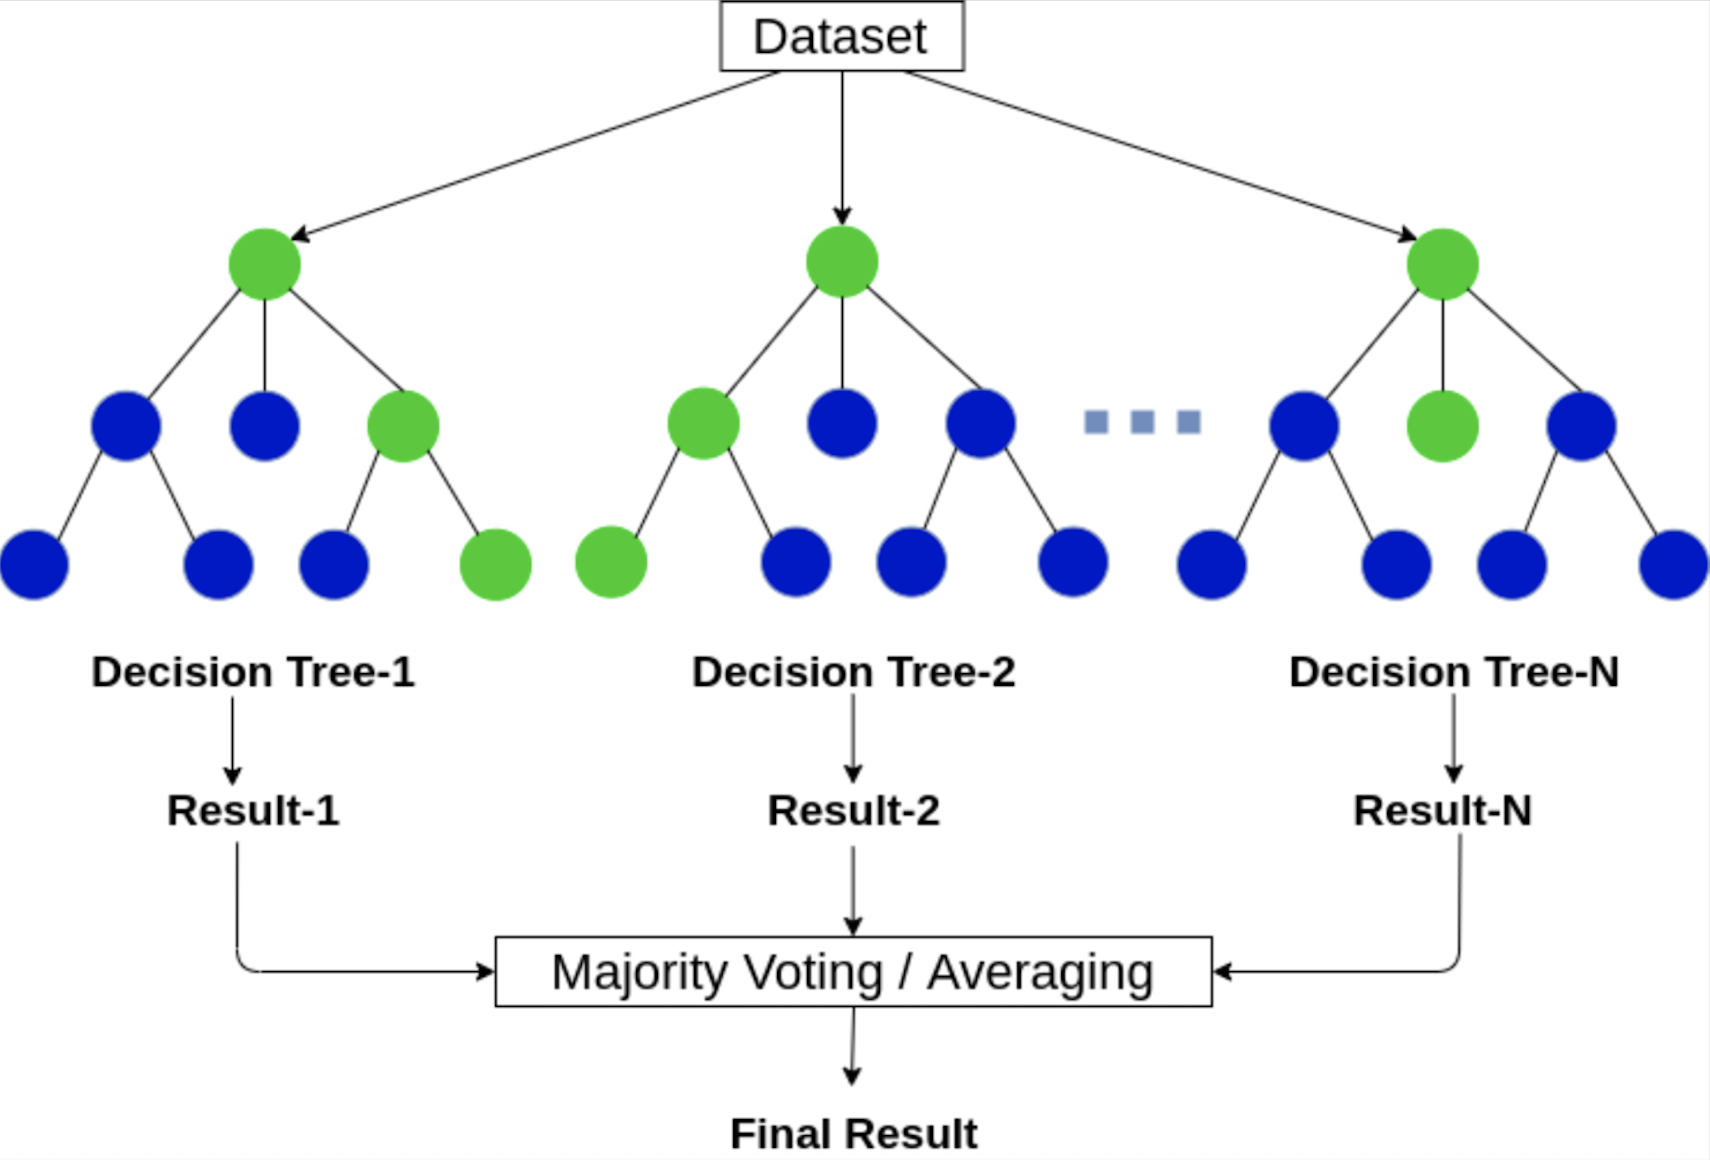
\includegraphics[width = 0.7\columnwidth]{figures/tree.png}
    \caption{Illustration of a RF (source: analyticsvidhya.com)}
    \label{fig:my_label}
\end{figure}

\todo[inline]{More explanation on RF}

\subsubsection{RF simulation 1: 2 features}

We use the same data generated in section \ref{para_model}, and this time we calculate DR estimators with various nuisance parameter estimation settings that use logistic regression or RFs:
\begin{itemize}
    \item \texttt{DR logistic ps, forest om}: the propensity is a correctly specified logistic regression, and the outcome model is a RF. Both model account for the interaction term between $W_1$ and $W_2$ in feature engineering.
    \item \texttt{DR logistic om, forest ps}: the outcome model is a correctly specified logistic regression, and the propensity score is a RF.
    \item \texttt{DR forest}: both the propensity and the outcome model are RFs that account for the interaction term between $W_1$ and $W_2$ in feature engineering.
    \item \texttt{DR wrong logistic om, forest ps}: the outcome model is an incorrectly specified logistic regression, and the propensity score is a correctly specified RF.
    \item \texttt{DR wrong logistic ps, forest om}: the propensity is an incorrectly specified logistic regression, and the outcome model is a correctly specified RF.
    \item \texttt{DR wrong forest om, forest ps}: the outcome model is an incorrectly specified RF (i.e no interaction term in feature engineering), and the propensity score is a correctly specified RF.
    \item \texttt{DR wrong forest ps, forest om}: the propensity is an incorrectly specified RF (i.e no interaction term in feature engineering), and the outcome model is a correctly specified RF.
    \item \texttt{DR wrong forest ps \& om}: both the propensity and the outcome model are incorrectly specified RFs in feature engineering.
    \item \texttt{DR exact}: both the propensity and outcome model are exactly specified by using the distributions from the data generative methods, added for comparison.
\end{itemize}

Each time a RF is specified, it goes through a stratified 5-fold cross validation of RF parameters in order to input the parameters that give a RF with the best accuracy on the test sets. A summary of the parameters tested by the cross-validation is provided in table \ref{tableRF}.\\
\begin{table}[]
    \centering
\begin{tabular}{ |p{3cm}|p{3cm}|p{3cm}| }
 \hline
 \multicolumn{3}{|c|}{RF Cross-validation: Parameter Grid} \\
 \hline
 Number of decision trees & Maximum tree depth (number of splits)  & Maximum    number of features considered at each branch split\\
 \hline
 600, 800, 1000& 10, 15, 20, 25, 30 & 1, 2 \\
 \hline 
\end{tabular}
\caption{Parameter grid of 5-fold cross-validation for RFs in simulation 1}
\label{tableRF}
\end{table}

As before, we obtain an empirical bias by taking the sample mean of 2500 generated estimators of each sample size varying from 200 to 1200 rows. 

\subsubsection*{Results}

\todo[inline]{missing sample size N = 1200, 1400}
\begin{figure}[h!]
    \centering
    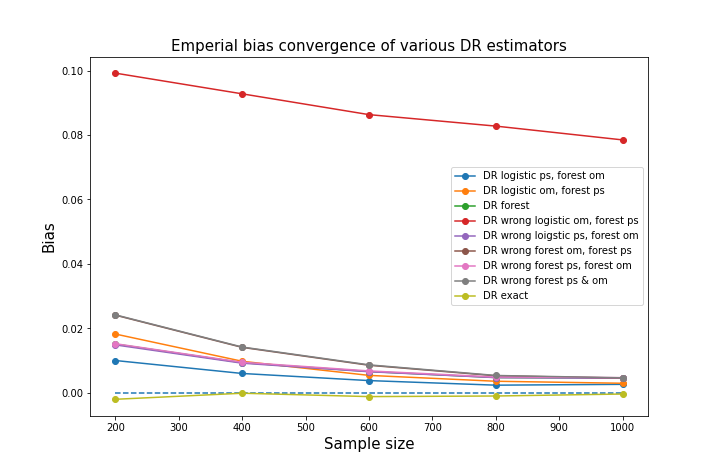
\includegraphics[width = 0.9\columnwidth]{figures/biasRF.png}
    \caption{RF simulation 1 results of bias for the various DR estimator specifications}
    \label{figbiasRF}
\end{figure}

\begin{figure} 
    \centering
    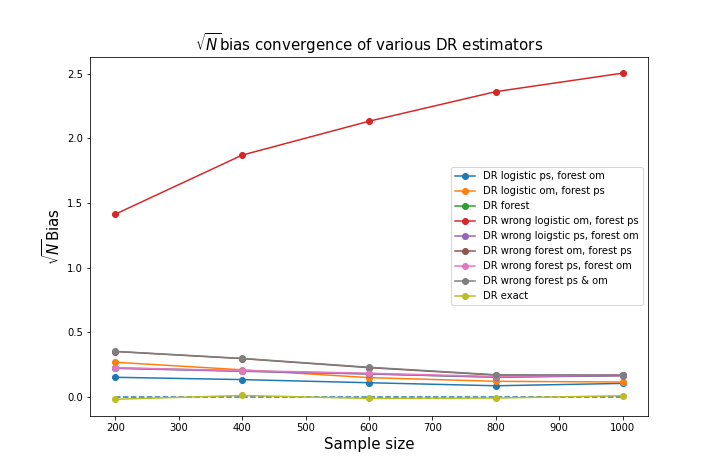
\includegraphics[width = 0.9\columnwidth]{figures/sqrtnRF.png}
    \caption{RF simulation 1 results of $\sqrt{N}$bias for the various DR estimator specifications}
    \label{figsqrtnRF}
\end{figure}

We notice in figure \ref{figbiasRF} that the models with RF still provide DR estimates that have bias converging to 0, even when the propensity and outcome model are set using a RF that doesn't account for the interaction term. This suggests that the RF is able to recover the misspecification, making it a useful tool in setting the nuisance parameters. Based on the sample sizes considered, figure \ref{figsqrtnRF} also suggests that theses models have biases with rate of convergence to 0 faster than $N^{-1/2}$, which further illustrates the double robustness of the estimator.

We also notice that when the outcome model was a RF and the propensity was wrongly specified with a model that doesn't account for the interaction term, whether that was a logistic regression or a RF, the bias still performs well, which is in line with what \citet{ps_SL} have shown about the recovery of unbiasedness with ML tools for the outcome model when dealing with a wrong propensity score. 

However these figures show an unusual result for the model that had a wrong logistic outcome model, paired with a RF propensity score. As we can see in figure \ref{figsqrtnRF}, the bias of this estimate does not converge fast enough, as the plot suggest its rate of convergence to 0 is slower than $N^{-1/2}$, making this estimate inconsistent, whereas when the misspecification of the outcome model is through a RF, the bias still performs well (its brown line on the graph is overlapped with the grey line). This makes us wonder if a RF on the propensity is not strong enough to recover the parametric misspecification of the outcome model.

As for the CI coverage results of the various DR estimations in figure \ref{figCIRF}, we notice that their convergence is slower compared to the parametric setting in section \ref{para_model}, and perhaps getting results from larger sample sizes would have shown that they eventually reach the 95\% goal. Figure \ref{figSERF} shows that the standard deviation of the estimated means also converge to the estimated value of the SE at a slower rate than the parametric setting, hence explaining the slowness in CI coverage convergence as well. However for the DR estimator with the wrong logistic outcome model and RF propensity, this CI coverage simply converges to 0 (with the SE estimate diverging from the standard deviation in \ref{figSERF}), so we eventually don't contain the true value of the sample mean in the CIs based on this specification of the DR estimator. Again, more exploration of DR estimations using a wrong parametric outcome model and a RF propensity is needed to see why this phenomenon is happening.

\begin{figure}[h!]
    \centering
    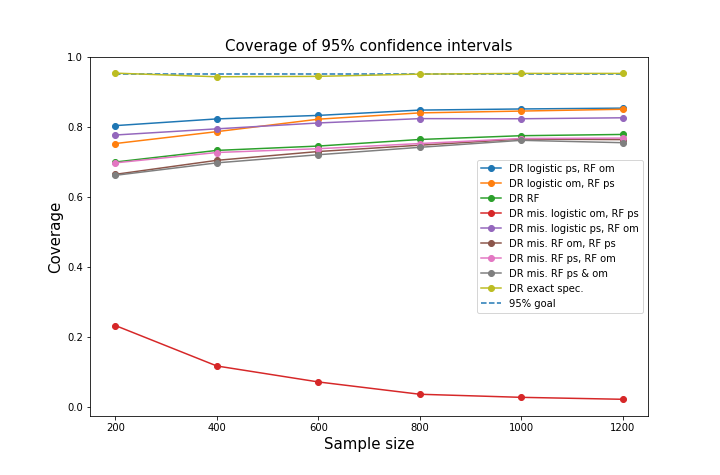
\includegraphics[width = 0.9\columnwidth]{figures/CIRF.png}
    \caption{RF simulation 1 results of 95\% CIs coverage for the various DR estimator specifications}
    \label{figCIRF}
\end{figure}

Going back to the DR estimates that were only specified with RFs, figure \ref{fighistRF} suggest asymptotic normality of the distribution of these estimates, like in the parametric setting. \\

Overall the use of RFs in this data setting has resulted in consistent DR estimates (with the exception of one estimate mentioned before). Moreover, misspecification of the models by omitting the interaction term was an issue that the RFs easily overcame, as seen in the similar consistency and asymptotic normality results of the RF models that did and did not account for this interaction. This is a non-negligible upgrade from the parametric setting as it suggests that RFs can provide a sort of safety cushion for model specification.

\begin{figure}[h!]
    \centering
    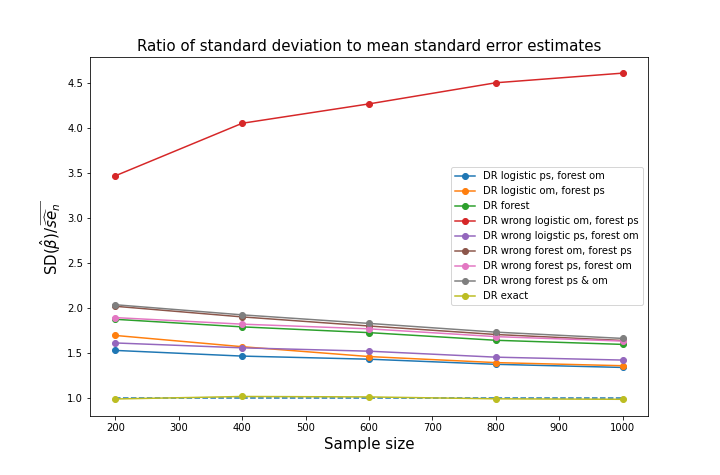
\includegraphics[width = 0.9\columnwidth]{figures/SERF.png}
    \caption{RF simulation 1's accuracy of \citet{lunceford_davidian} SE estimation for the various DR estimator specifications}
    \label{figSERF}
\end{figure}

\begin{figure}[h!]
    \centering
    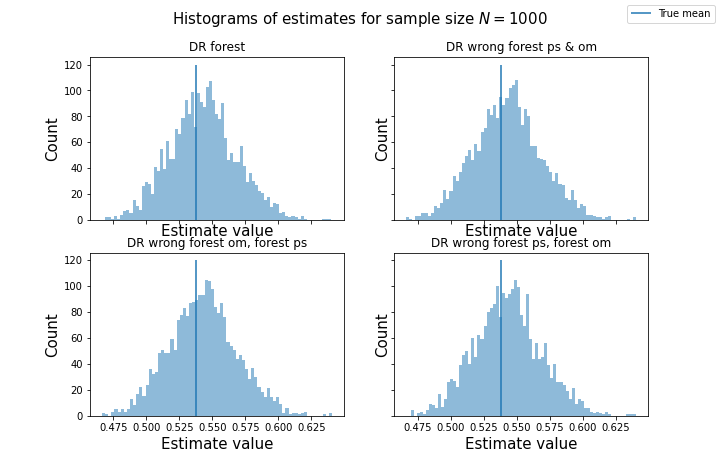
\includegraphics[width = 0.9\columnwidth]{figures/histRF.png}
    \caption{RF simulation 1's histograms of DR estimates for sample size $N = 1000$}
    \label{fighistRF}
\end{figure}

\clearpage
\subsubsection{RF simulation 2: 4 features}

This time we increase the complexity of our DR estimation by adding two new features to the data-generative method from the previous section. We now have $\mathbf{W} = (W_1,W_2,W_3,W_4)$ where $W_1,W_2$ are as before, $W_3$ follows a standard normal distribution and $W_4$ follows an exponential distribution with mean 1. The features are mutually independent. The new true propensity score is 
\begin{align*}
    \pi(\mathbf{W}) = P(R = 1 |\mathbf{W} = (w_1,w_2, w_3,w_4)) = \expit(-w_1 + 2w_1w_2 - w_3 + 2w_3w_4)
\end{align*}
and the new true outcome model is 
\begin{align*}
    m(\mathbf{W}) &= E(Y|\mathbf{W}, R=1) \\
    & = \expit(0.2 - w_1 + 2w_1w_2 - w_3 + 2w_3w_4)
\end{align*}

We ran simulations using the same combination of nuisance parameter settings as in simulation 1 with 2 features, but this time when we refer to wrong specification, it means the model didn't account for both interaction terms $W_1W_2$ and $W_3W_4$. The cross-validation for the RFs was also expanded so as to consider up to 4 features at a time in each split. 

\subsubsection*{Results}

\todo[inline]{missing sample size N = 1400}
Unlike the simulation with 2 features, this time with the addition of 2 new features we obtained estimates that had poor convergence rates. Figure \ref{figbiasRF_moreW} already suggests higher bias in the estimators and a deceleration of the bias rate of convergence compared to the simulation with 2 features. This is further illustrated in figure \ref{figsqrtnRF_moreW} as the divergence of the bias elevated to $N^{1/2}$ suggest that the rate of convergence to 0 is slower than $N^{-1/2}$. The only estimator that performed well in this setting, based on the sample sizes considered, is the estimator with a correct logistic outcome model and a RF propensity score that accounts for the interactions terms (orange line in the plots). 

\begin{figure}[h!]
    \centering
    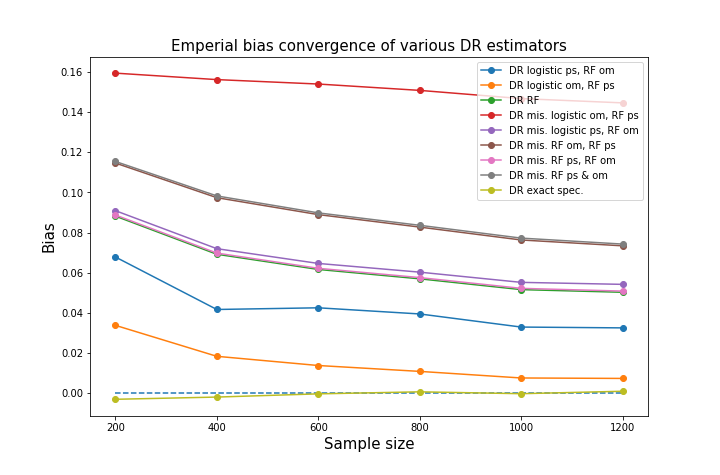
\includegraphics[width = 0.9\columnwidth]{figures/biasRF_moreW.png}
    \caption{RF simulation 2 results of bias for the various DR estimator specifications}
    \label{figbiasRF_moreW}
\end{figure}

\begin{figure}[h!]
    \centering
    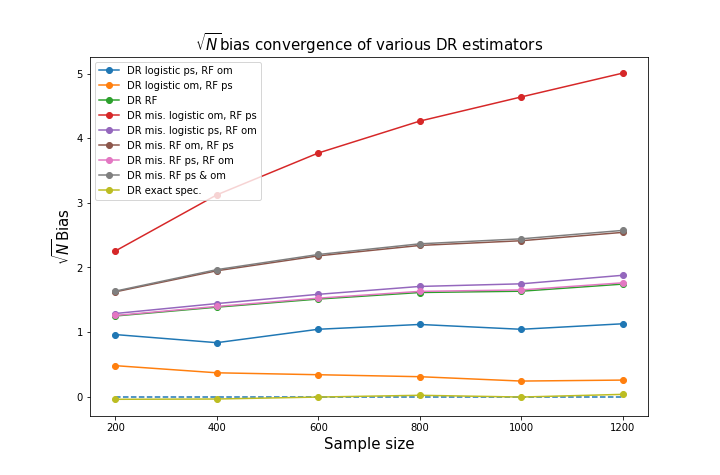
\includegraphics[width = 0.9\columnwidth]{figures/sqrtnRF_moreW.png}
    \caption{RF simulation 2 results of $\sqrt{N}$bias for the various DR estimator specifications}
    \label{figsqrtnRF_moreW}
\end{figure}

Unsurprisingly, the convergence to 95\% CI coverage is also poor as seen in figure \ref{figCIRF_moreW}, and in fact many of the estimators have a CI coverage converging to 0. This is further illustrated by the divergence of the SE estimate from the true deviation as seen in figure \ref{figSERF_moreW}. Even for the estimator that had a fast enough bias convergence (orange in plots), the convergence to a 95\% coverage of its CIs is relatively slow, and from sample size 1000 to 1200, there is a slight decrease in coverage. This might suggest a worsening of the CI coverage in larger samples.

\begin{figure}[h!]
    \centering
    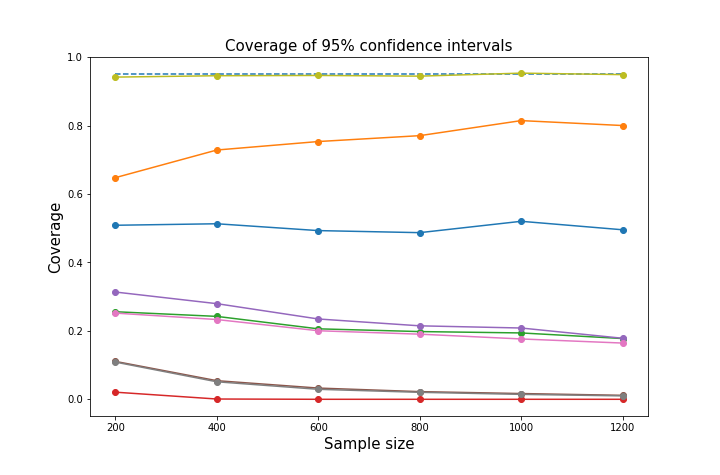
\includegraphics[width = 0.9\columnwidth]{figures/CIRF_moreW.png}
    \caption{RF simulation 2 results of 95\% CIs coverage for the various DR estimator specifications}
    \label{figCIRF_moreW}
\end{figure}

\begin{figure}[h!]
    \centering
    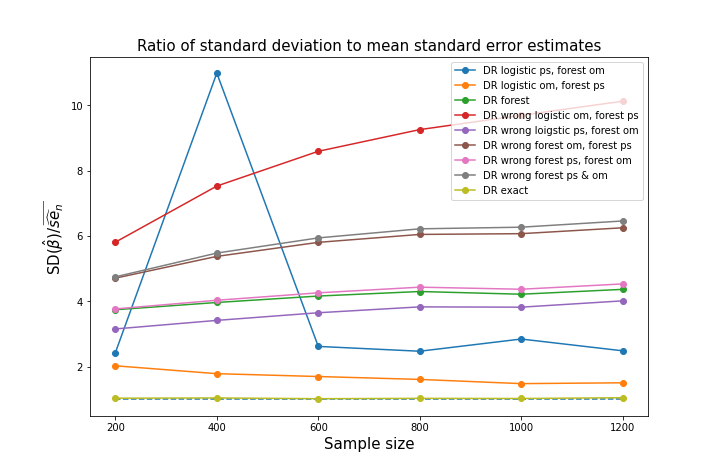
\includegraphics[width = 0.9\columnwidth]{figures/SERF_moreW.png}
    \caption{RF simulation 2's accuracy of \citet{lunceford_davidian} SE estimation for the various DR estimator specifications}
    \label{figSERF_moreW}
\end{figure}

It is with no surprise that due to the slowness of the convergences, a normal distribution centered at the true mean hasn't been achieved for the largest sample size considered in the simulation, in particular for the DR estimators involving RFs only, as seen in figure \ref{fighistRF_moreW}. \\

\begin{figure}[h!]
    \centering
    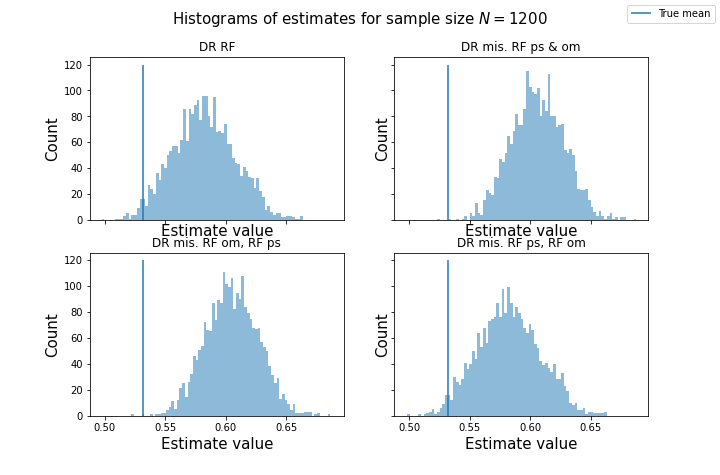
\includegraphics[width = 0.9\columnwidth]{figures/histRF_moreW.png}
    \caption{RF simulation 2's histograms of DR estimates for sample size $N = 1200$}
    \label{fighistRF_moreW}
\end{figure}

Overall, doubling the number of features has resulted in poor bias and slow convergence of the DR estimates to the true value of the mean. This may be an example of the so-called curse of dimensionality \citep{Wasserman2006}: by doubling the number of features, the complexity of training the RFs overcomes correct classification or regression, leading to the poor convergence of our DR estimates to the true value. Had the added features $W_3,W_4$ had a smaller range of values, we might have alleviated the complexity of the classification problem. Although we had found good results using RFs in the 2-features case, one must take into account the complexity of the dataset and classification/regression problem before choosing to use a RF to set the nuisance parameters of a DR estimator.

\clearpage
\subsection{Using MLPs}
\begin{figure}[h!]
    \centering
    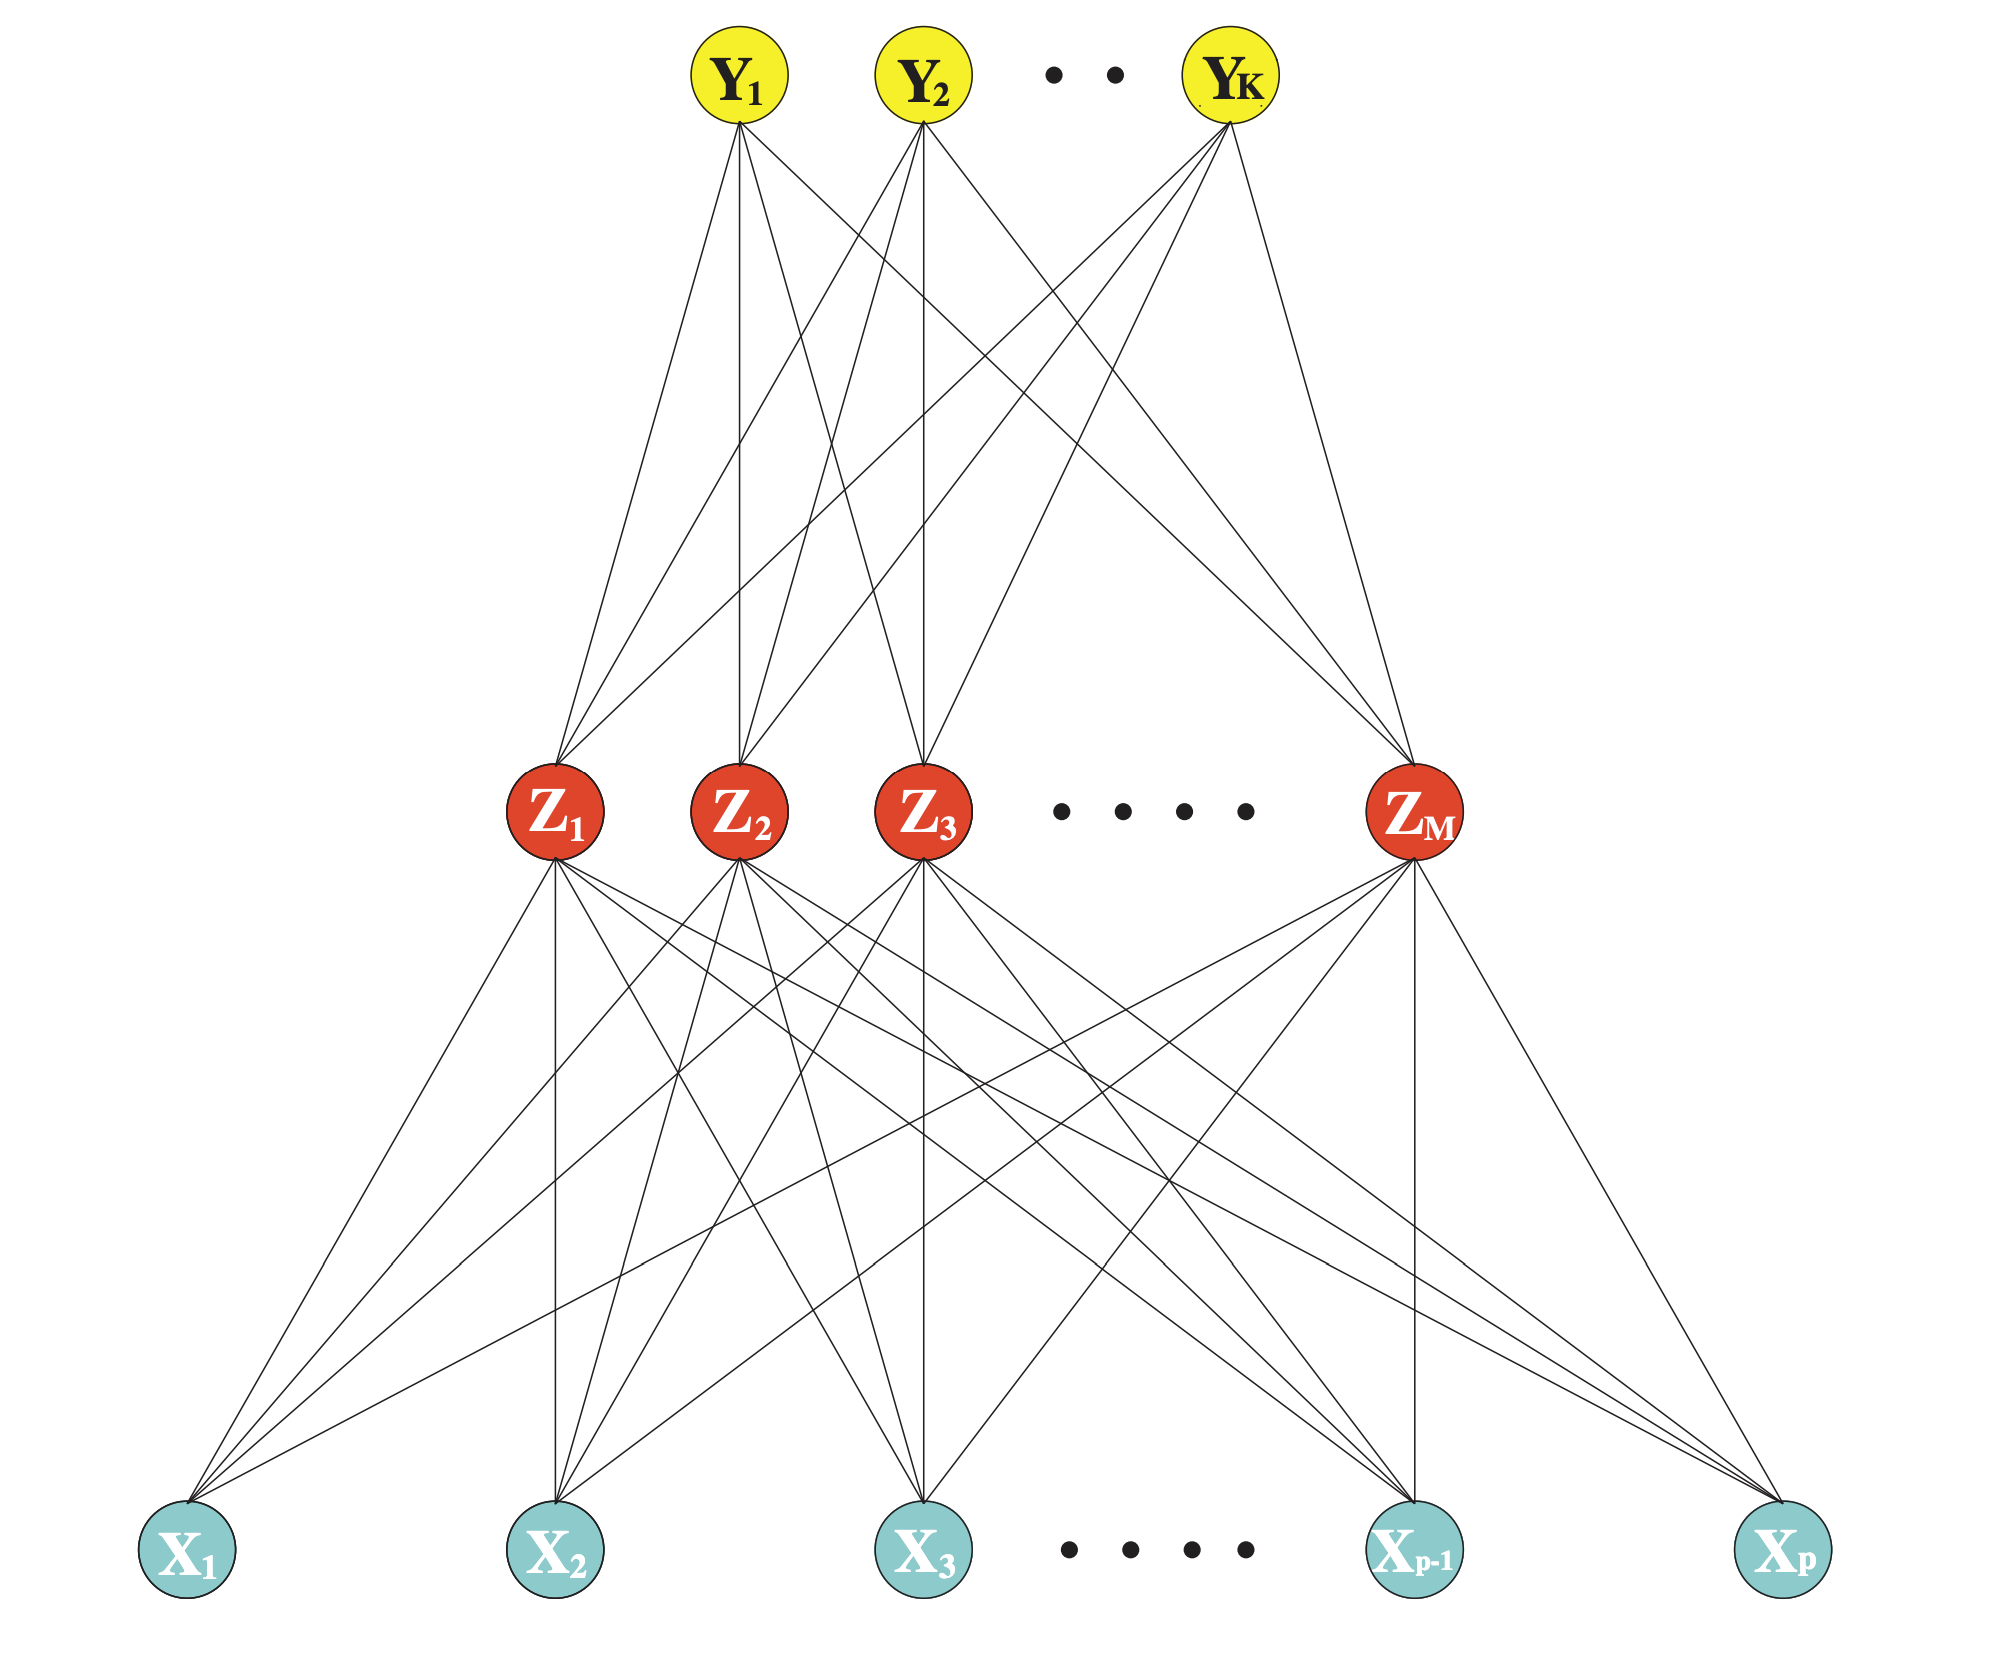
\includegraphics[width = 0.7\columnwidth]{figures/Screenshot 2021-05-26 at 19.21.43.png}
    \caption{Network diagram of a single layer perceptron, \citet{hastieESL}}
    \label{fignn}
\end{figure}

This section is motivated by the publication by \citet{setoguchi-nn} suggesting that neural networks reduce the bias of propensity scores compared to logistic regression, and hence should also alleviate the bias of the DR estimator. This time we are using MLPs, a type of forward-feeding artificial neural network. As mentioned by \citet{hastieESL}, there is a lot of popularity surrounding neural networks lately, and like RFs, they are easy to implement in Python thanks to the scikit-learn module. The training time of a MLP is also faster than that of a RF for models with a small number of features. 

In a classification problem, there are $K$ output nodes at the end of the network diagram corresponding to the $K$ categories the output $Y$ can be in. The first layer of nodes in the diagram corresponds to the $p$ input features. Then, each node in the hidden layers of the network is created as a linear combination of the previous layer's nodes. At the end of the network, the output nodes are created as functions of linear combinations of the last hidden layer's nodes. An illustration of the network diagram of a single layer perceptron is provided in figure \ref{fignn}, taken from \textit{The Elements of Statistical Learning} by \citet{hastieESL}.

In the following sections we will evaluate the use of MLPs for DR estimation, through simulations on the data setting we have encountered in the previous sections.

\subsubsection{MLP simulation 1: 2 features}

We go back to the data structure that had 2 features $W_1,W_2$, and we wish to see what happens to the consistency of the DR estimates when we use MLPs for the propensity score or outcome model. The various DR estimates based on MLP nuisance parameters are as follows: 
\begin{itemize}
    \item \texttt{DR logistic ps, MLP om}: the propensity is a correctly specified logistic regression, and the outcome model is a MLP. Both model account for the interaction term between $W_1$ and $W_2$
    \item \texttt{DR logistic om, MLP ps}: the outcome model is a correctly specified logistic regression, and the propensity score is a MLP.
    \item \texttt{DR MLP}: both the propensity and the outcome model are MLPs that account for the interaction term between $W_1$ and $W_2$.
    \item \texttt{DR wrong logistic om, MLP ps}: the outcome model is an incorrectly specified logistic regression, and the propensity score is a correctly specified MLP.
    \item \texttt{DR wrong logistic ps, MLP om}: the propensity is an incorrectly specified logistic regression, and the outcome model is a correctly specified MLP.
    \item \texttt{DR wrong MLP om, MLP ps}: the outcome model is an incorrectly specified MLP (i.e no interaction term), and the propensity score is a correctly specified MLP.
    \item \texttt{DR wrong MLP ps, MLP om}: the propensity is an incorrectly specified MLP (i.e no interaction term), and the outcome model is a correctly specified MLP.
    \item \texttt{DR wrong MLP ps \& om}: both the propensity and the outcome model are incorrectly specified MLPs.
    \item \texttt{DR exact}: both the propensity and outcome model are exactly specified by using the distributions from the data generative methods, added for comparison.
\end{itemize}

Like with RFs, the MLPs also go through a 5-fold cross-validation process to tune model parameters. A summary of the range of parameters tested by the cross-validation is provided in table \ref{tableMLP}.

\begin{table}[h!]
    \centering
\begin{tabular}{ |p{3cm}|p{3cm}|p{3cm}|p{3cm}| }
 \hline
 \multicolumn{4}{|c|}{MLP Cross-validation: Parameter Grid} \\
 \hline
 Hidden layer sizes & Learning rate & Activation & Alpha\\
 \hline
 3 layers of size (10, 20, 30), 2 layers of size (50, 50), 1 layer of size 100 & Constant, invscaling, adaptive & Logistic, relu, tanh & $10^{-1}$, $10^{-2}$, $10^{-3}$, $10^{-4}$ \\
 \hline 
\end{tabular}
\caption{Parameter grid of 5-fold cross-validation for MLPS in simulation 1}
\label{tableMLP}
\end{table}

\subsubsection*{Results}

\begin{figure}[h!]
    \centering
    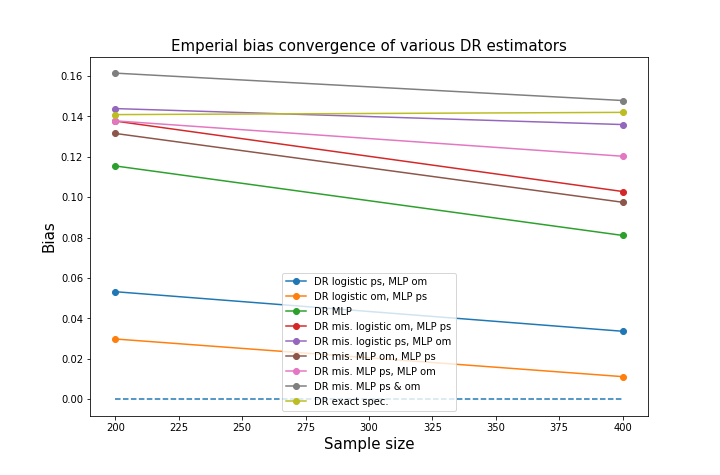
\includegraphics[width = 0.9\columnwidth]{figures/biasMLP.png}
    \caption{MLP simulation 1 results of bias for the various DR estimator specifications}
    \label{figbiasMLP}
\end{figure}

\begin{figure}[h!]
    \centering
    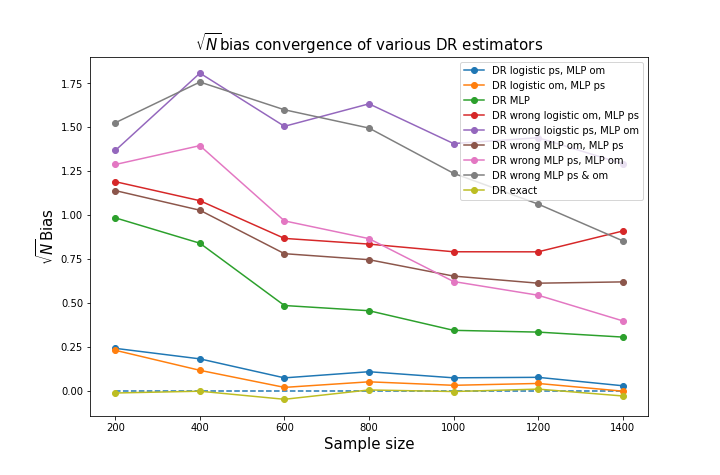
\includegraphics[width = 0.9\columnwidth]{figures/sqrtnMLP.png}
    \caption{MLP simulation 1 results of $\sqrt{N}$bias for the various DR estimator specifications}
    \label{figsqrtnMLP}
\end{figure}

In figure \ref{figbiasMLP} we notice that most estimates involving at least one MLP nuisance parameters have a bias seeming to converge towards zero. Excluding the DR estimate with exact specification, the estimate with lowest bias is the one that had a logistic outcome regression and a MLP propensity score, and it outperforms the estimate with logistic propensity score. This goes in line with the findings of \citet{setoguchi-nn} about an MLP propensity score having lower bias than with logistic regression. The DR estimate set with correct MLPs for both nuisance parameters performs well in terms of bias as well, although the convergence to 0 bias plateaus as sample sizes get larger. The DR estimate with wrong logistic outcome model and MLP propensity score (red line in plot) has a U-shaped bias curve, suggesting a worsening bias in larger samples. Looking at figure \ref{figsqrtnMLP}, the bias convergence to 0 for these estimates seem to be faster than that of $N^{-1/2}$ for most estimates as shown by the downward trend of the $\sqrt{N}$bias curves, while the estimate with wrong logistic outcome model and propensity MLP shows sign of diverging, in line with what we saw in figure \ref{figbiasMLP}. The DR estimator with wrong logistic propensity score and MLP outcome model, \texttt{DR wrong logistic ps, MLP om} (purple line on the plots) has one of highest bias among these estimators, but the convergence of the bias at a higher speed than $N^{-1/2}$ suggests that the incorrect specification was overcome by the MLPs and so the estimate is still consistent, even though it will converge towards the true mean at a slower pace than the estimates with at least one correct MLP specification. Another notable estimate is the one with wrong MLP propensity and MLP outcome model (pink line in plots). Even though this estimate starts at high bias, the latter is seeming to quickly converge to 0.

\begin{figure}[h!]
    \centering
    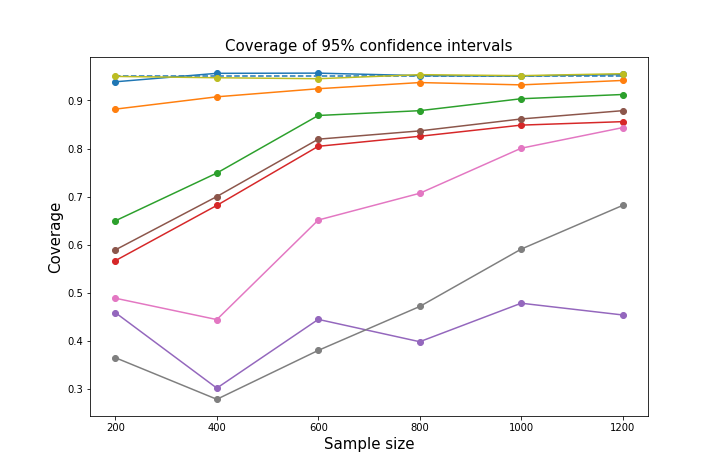
\includegraphics[width = 0.9\columnwidth]{figures/CIMLP.png}
    \caption{MLP simulation 1 results of 95\% CIs coverage for the various DR estimator specifications}
    \label{figCIMLP}
\end{figure}

The CI coverage plot in figure \ref{figCIMLP} also show interesting results. \texttt{DR logistic om, MLP ps}, \texttt{DR logistic ps, MLP om}, \texttt{DR wrong MLP om, MLP ps} and \texttt{DR wrong MLP ps \& om} (in blue, orange pink and grey) have CI coverage tending to the 95\% goal, with the estimates with higher bias generally tending to 95\% coverage at a slower rate. Their SE estimates, as seen \ref{figSEMLP}, also suggest to be tending towards the true value. On the other hand, we see a upside down U-shape from the CI coverage and SE estimate curves of \texttt{DR MLP, DR logistic om, MLP ps, DR wrong MLP om, MLP ps} (in green, red and brown), suggesting a worsening CI coverage for larger sample sizes. These plots seem to suggest that a misspecification of the MLP for the propensity score is actually providing a better CI coverage convergence of the DR estimates. The DR estimate struggling to get up to high CI coverage the most here is again \texttt{DR wrong logistic ps, MLP om}. We see from figure \ref{figSEMLP} that non-surprisingly, its SE estimate is converging to the true standard deviation at a slow pace as well, given the considered sample sizes. 

\begin{figure}[h!]
    \centering
    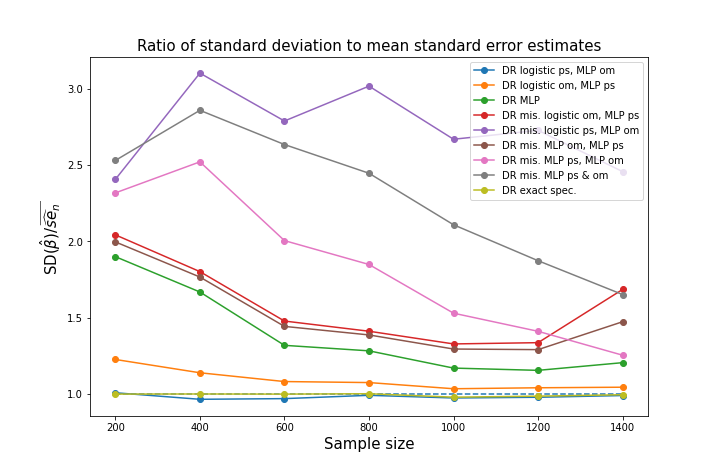
\includegraphics[width = 0.9\columnwidth]{figures/SEMLP.png}
    \caption{MLP simulation 1's accuracy of \citet{lunceford_davidian} SE estimation for the various DR estimator specifications}
    \label{figSEMLP}
\end{figure}

\begin{figure}[h!]
    \centering
    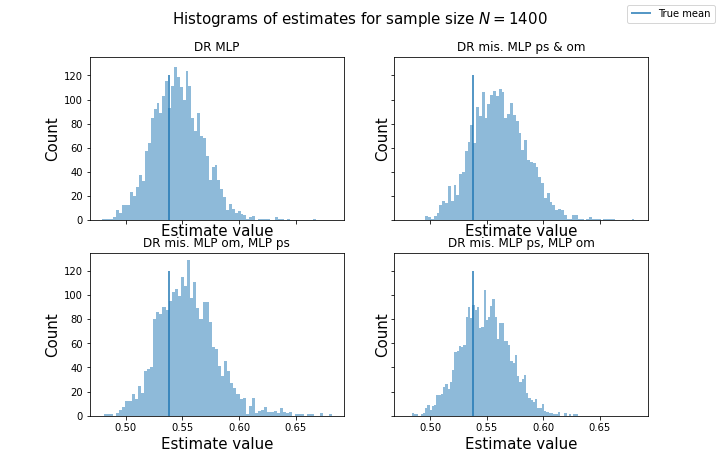
\includegraphics[width = 0.9\columnwidth]{figures/histMLP.png}
    \caption{MLP simulation 1's histograms of DR estimates for sample size $N = 1200$}
    \label{fighistMLP}
\end{figure}

Taking a particular look at the histograms of the DR estimates involving only MLPs for the largest sample size considered, we notice that although \texttt{DR MLP} and \texttt{DR wrong MLP om, MLP ps} have distributions almost centered at the true mean, we know from the diverging trend of their CI coverage at larger samples that these histogram will be less and less centered at the true mean as we increase sample size, so we wouldn't expect asymptotic normality from these. On the other hand, from the way the bias and CI coverage of \texttt{DR wrong MLP ps \& om} and \texttt{DR wrong MLP ps, MLP om} were converging, we are likely to get asymptotic normal distribution from these estimates, although at a slower rate than the parametric setting. Since \texttt{DR wrong MLP ps \& om} had higher bias, its histogram in figure \ref{fighistMLP} is less centered at the true value than that of \texttt{DR wrong MLP ps, MLP om} at the given sample size. One would expect to see better centering of these histogram, had a larger sample size been considered.
\clearpage
\subsubsection{MLP simulation 2: 4 features}

\todo[inline]{to be added once results come back}

\clearpage
\subsection{Discussion}
\todo[inline]{missing sample size N = 1200, 1400}
\begin{figure}[h!]
    \centering
    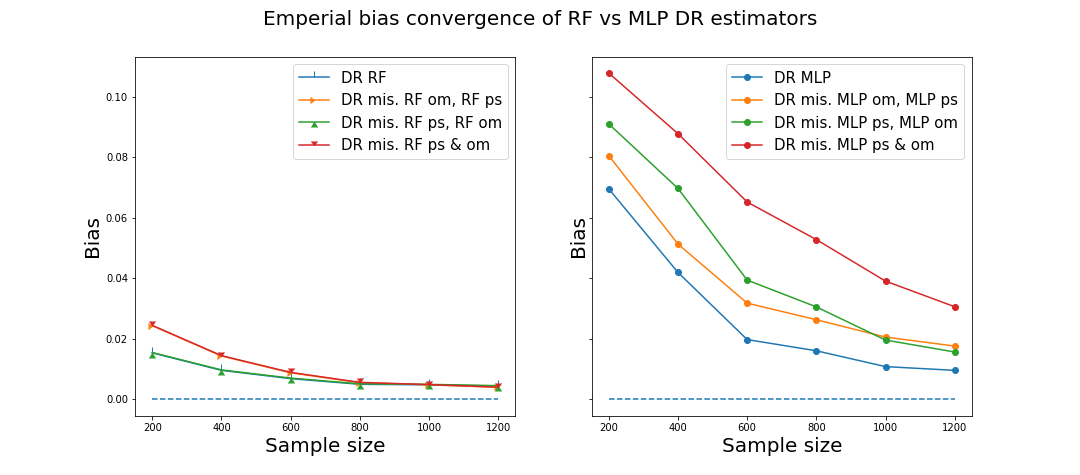
\includegraphics[width = 0.8\columnwidth]{figures/biascompare.png}
    \caption{Comparing bias performance on simulation with 2 features}
    \label{fig:my_label}
\end{figure}

\begin{figure}[h!]
    \centering
    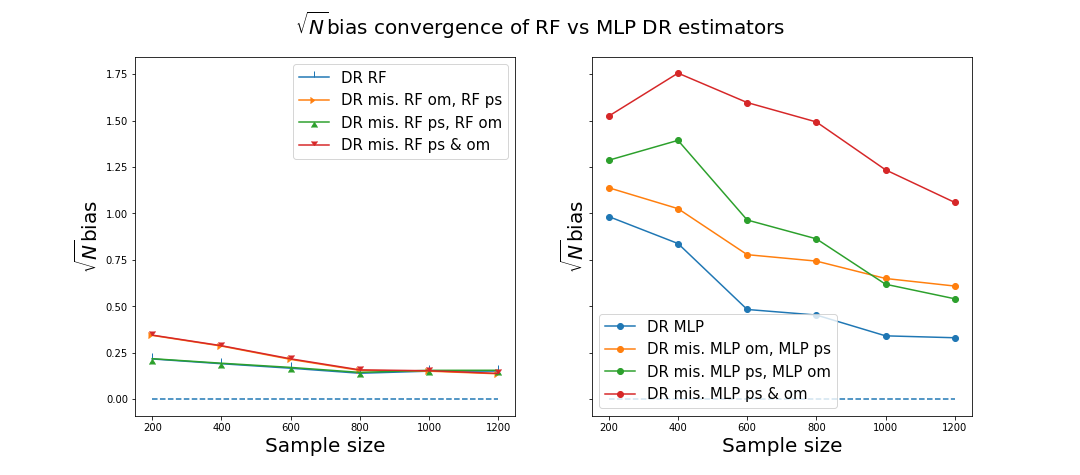
\includegraphics[width = 0.8\columnwidth]{figures/sqrtncompare.png}
    \caption{Caption}
    \label{fig:my_label}
\end{figure}

\todo[inline]{waiting for more results}

- RF gives lower bias but convergence rate is slow compared to MLP 

- RF: with/without interaction terms not an issue, MLP: without interaction for ps gives better convergence rates 

- why is bias diverging after some sample size for some MLPs?

- there might be issues of overfitting here since we train and test on 80\% data but fit on 100\%

- complexity of the data set has a lot of influence on these performances; continuous features = infinite input categories -> difficult to train classification model 

- more simulations on various data settings would be need to make more general remakrs on ML tools

- but ML tools = data adaptive so in real world scenario one would likely test a few tools and pick the one that give best ps / om fit on new data 

\section{Conclusion}

%% bibliography
\clearpage
\bibliographystyle{unsrtnat}
\bibliography{bibliography}

\clearpage
\section{Appendix}

\subsection*{Code for DR simulation}

\lstinputlisting[language=Python]{Code/DR_estimation.py}
\end{document}
